\documentclass[1p]{elsarticle_modified}
%\bibliographystyle{elsarticle-num}

%\usepackage[colorlinks]{hyperref}
%\usepackage{abbrmath_seonhwa} %\Abb, \Ascr, \Acal ,\Abf, \Afrak
\usepackage{amsfonts}
\usepackage{amssymb}
\usepackage{amsmath}
\usepackage{amsthm}
\usepackage{scalefnt}
\usepackage{amsbsy}
\usepackage{kotex}
\usepackage{caption}
\usepackage{subfig}
\usepackage{color}
\usepackage{graphicx}
\usepackage{xcolor} %% white, black, red, green, blue, cyan, magenta, yellow
\usepackage{float}
\usepackage{setspace}
\usepackage{hyperref}

\usepackage{tikz}
\usetikzlibrary{arrows}

\usepackage{multirow}
\usepackage{array} % fixed length table
\usepackage{hhline}

%%%%%%%%%%%%%%%%%%%%%
\makeatletter
\renewcommand*\env@matrix[1][\arraystretch]{%
	\edef\arraystretch{#1}%
	\hskip -\arraycolsep
	\let\@ifnextchar\new@ifnextchar
	\array{*\c@MaxMatrixCols c}}
\makeatother %https://tex.stackexchange.com/questions/14071/how-can-i-increase-the-line-spacing-in-a-matrix
%%%%%%%%%%%%%%%

\usepackage[normalem]{ulem}

\newcommand{\msout}[1]{\ifmmode\text{\sout{\ensuremath{#1}}}\else\sout{#1}\fi}
%SOURCE: \msout is \stkout macro in https://tex.stackexchange.com/questions/20609/strikeout-in-math-mode

\newcommand{\cancel}[1]{
	\ifmmode
	{\color{red}\msout{#1}}
	\else
	{\color{red}\sout{#1}}
	\fi
}

\newcommand{\add}[1]{
	{\color{blue}\uwave{#1}}
}

\newcommand{\replace}[2]{
	\ifmmode
	{\color{red}\msout{#1}}{\color{blue}\uwave{#2}}
	\else
	{\color{red}\sout{#1}}{\color{blue}\uwave{#2}}
	\fi
}

\newcommand{\Sol}{\mathcal{S}} %segment
\newcommand{\D}{D} %diagram
\newcommand{\A}{\mathcal{A}} %arc


%%%%%%%%%%%%%%%%%%%%%%%%%%%%%5 test

\def\sl{\operatorname{\textup{SL}}(2,\Cbb)}
\def\psl{\operatorname{\textup{PSL}}(2,\Cbb)}
\def\quan{\mkern 1mu \triangleright \mkern 1mu}

\theoremstyle{definition}
\newtheorem{thm}{Theorem}[section]
\newtheorem{prop}[thm]{Proposition}
\newtheorem{lem}[thm]{Lemma}
\newtheorem{ques}[thm]{Question}
\newtheorem{cor}[thm]{Corollary}
\newtheorem{defn}[thm]{Definition}
\newtheorem{exam}[thm]{Example}
\newtheorem{rmk}[thm]{Remark}
\newtheorem{alg}[thm]{Algorithm}

\newcommand{\I}{\sqrt{-1}}
\begin{document}

%\begin{frontmatter}
%
%\title{Boundary parabolic representations of knots up to 8 crossings}
%
%%% Group authors per affiliation:
%\author{Yunhi Cho} 
%\address{Department of Mathematics, University of Seoul, Seoul, Korea}
%\ead{yhcho@uos.ac.kr}
%
%
%\author{Seonhwa Kim} %\fnref{s_kim}}
%\address{Center for Geometry and Physics, Institute for Basic Science, Pohang, 37673, Korea}
%\ead{ryeona17@ibs.re.kr}
%
%\author{Hyuk Kim}
%\address{Department of Mathematical Sciences, Seoul National University, Seoul 08826, Korea}
%\ead{hyukkim@snu.ac.kr}
%
%\author{Seokbeom Yoon}
%\address{Department of Mathematical Sciences, Seoul National University, Seoul, 08826,  Korea}
%\ead{sbyoon15@snu.ac.kr}
%
%\begin{abstract}
%We find all boundary parabolic representation of knots up to 8 crossings.
%
%\end{abstract}
%\begin{keyword}
%    \MSC[2010] 57M25 
%\end{keyword}
%
%\end{frontmatter}

%\linenumbers
%\tableofcontents
%
\newcommand\colored[1]{\textcolor{white}{\rule[-0.35ex]{0.8em}{1.4ex}}\kern-0.8em\color{red} #1}%
%\newcommand\colored[1]{\textcolor{white}{ #1}\kern-2.17ex	\textcolor{white}{ #1}\kern-1.81ex	\textcolor{white}{ #1}\kern-2.15ex\color{red}#1	}

{\Large $\underline{11a_{41}~(K11a_{41})}$}

\setlength{\tabcolsep}{10pt}
\renewcommand{\arraystretch}{1.6}
\vspace{1cm}\begin{tabular}{m{100pt}>{\centering\arraybackslash}m{274pt}}
\multirow{5}{120pt}{
	\centering
	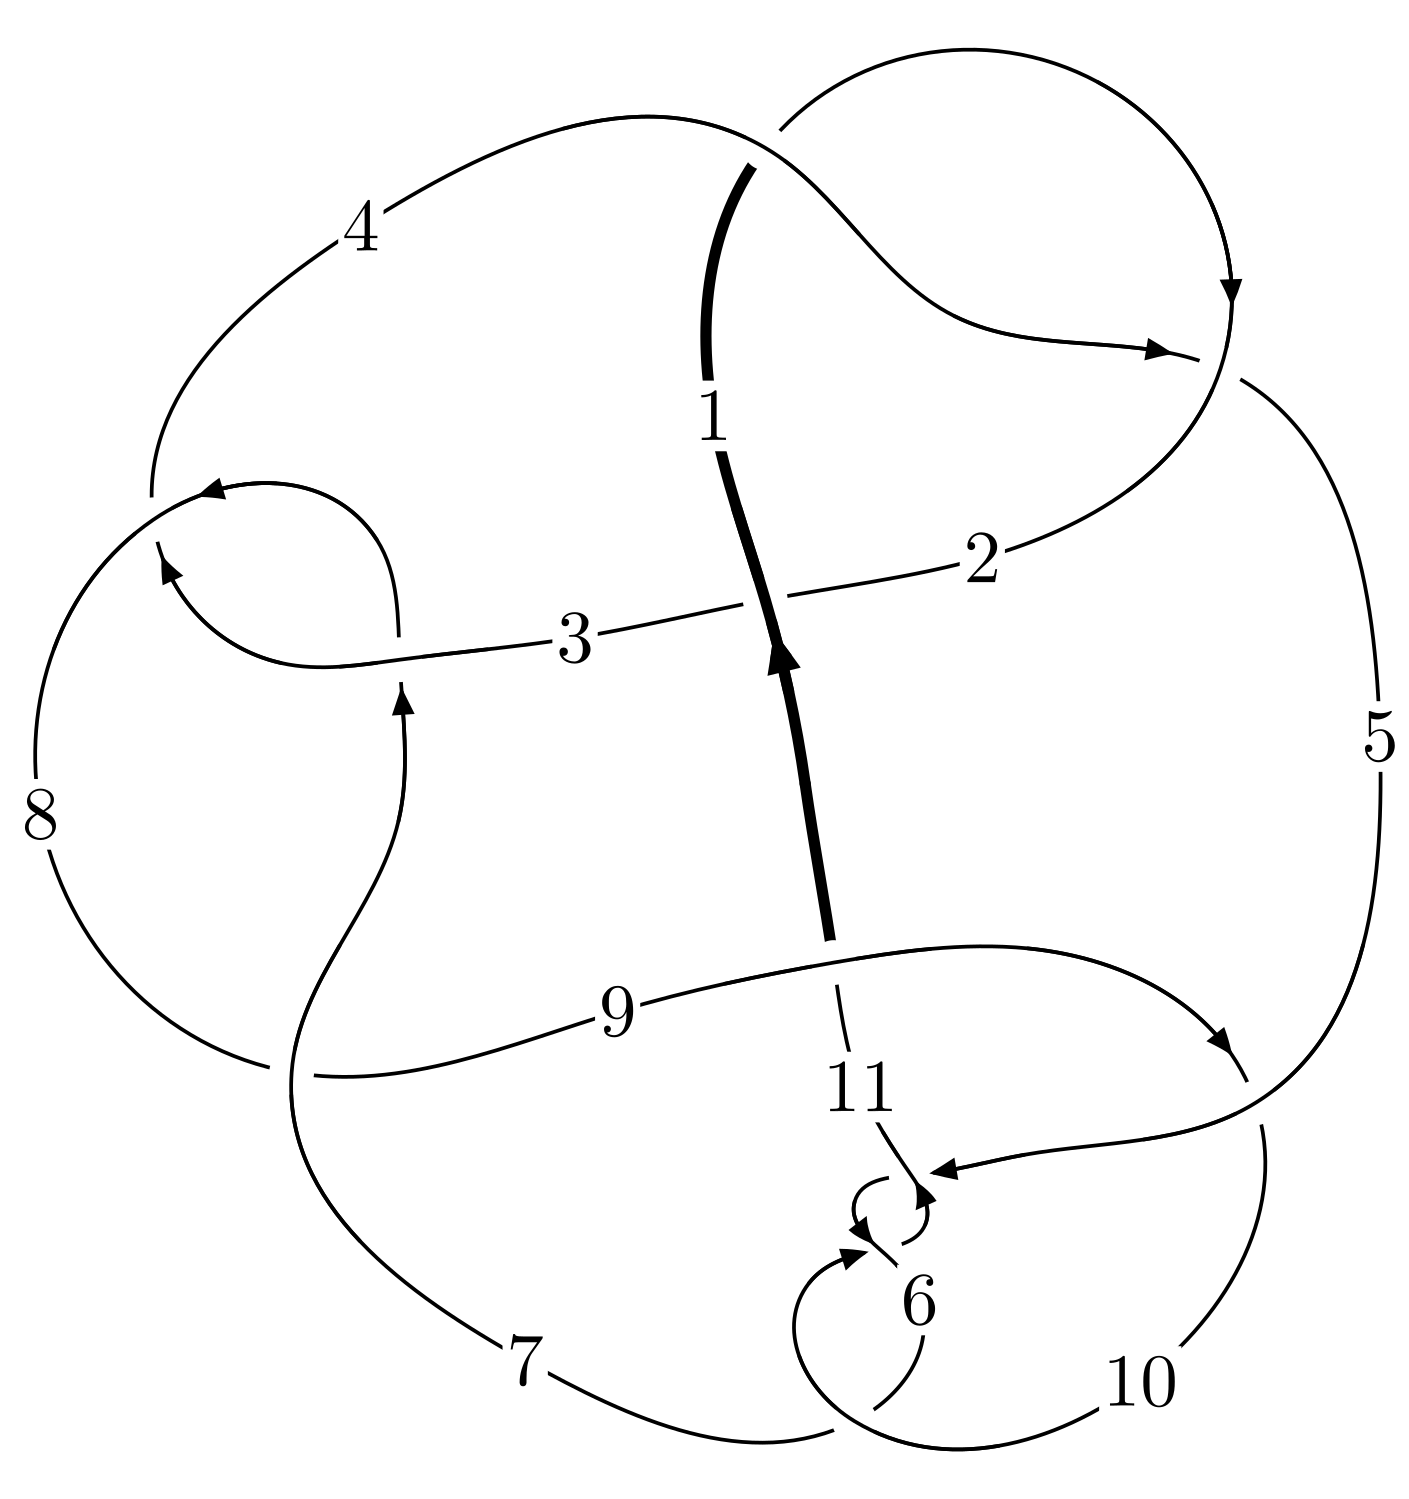
\includegraphics[width=112pt]{../../../GIT/diagram.site/Diagrams/png/290_11a_41.png}\\
\ \ \ A knot diagram\footnotemark}&
\allowdisplaybreaks
\textbf{Linearized knot diagam} \\
\cline{2-2}
 &
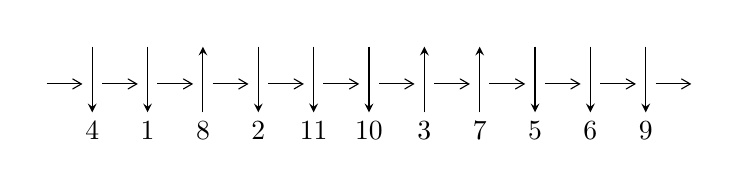
\begin{tikzpicture}[x=20pt, y=17pt]
	% nodes
	\node (C0) at (0, 0) {};
	\node (C1) at (1, 0) {};
	\node (C1U) at (1, +1) {};
	\node (C1D) at (1, -1) {4};

	\node (C2) at (2, 0) {};
	\node (C2U) at (2, +1) {};
	\node (C2D) at (2, -1) {1};

	\node (C3) at (3, 0) {};
	\node (C3U) at (3, +1) {};
	\node (C3D) at (3, -1) {8};

	\node (C4) at (4, 0) {};
	\node (C4U) at (4, +1) {};
	\node (C4D) at (4, -1) {2};

	\node (C5) at (5, 0) {};
	\node (C5U) at (5, +1) {};
	\node (C5D) at (5, -1) {11};

	\node (C6) at (6, 0) {};
	\node (C6U) at (6, +1) {};
	\node (C6D) at (6, -1) {10};

	\node (C7) at (7, 0) {};
	\node (C7U) at (7, +1) {};
	\node (C7D) at (7, -1) {3};

	\node (C8) at (8, 0) {};
	\node (C8U) at (8, +1) {};
	\node (C8D) at (8, -1) {7};

	\node (C9) at (9, 0) {};
	\node (C9U) at (9, +1) {};
	\node (C9D) at (9, -1) {5};

	\node (C10) at (10, 0) {};
	\node (C10U) at (10, +1) {};
	\node (C10D) at (10, -1) {6};

	\node (C11) at (11, 0) {};
	\node (C11U) at (11, +1) {};
	\node (C11D) at (11, -1) {9};
	\node (C12) at (12, 0) {};

	% arrows
	\draw[->,>={angle 60}]
	(C0) edge (C1) (C1) edge (C2) (C2) edge (C3) (C3) edge (C4) (C4) edge (C5) (C5) edge (C6) (C6) edge (C7) (C7) edge (C8) (C8) edge (C9) (C9) edge (C10) (C10) edge (C11) (C11) edge (C12) ;	\draw[->,>=stealth]
	(C1U) edge (C1D) (C2U) edge (C2D) (C3D) edge (C3U) (C4U) edge (C4D) (C5U) edge (C5D) (C6U) edge (C6D) (C7D) edge (C7U) (C8D) edge (C8U) (C9U) edge (C9D) (C10U) edge (C10D) (C11U) edge (C11D) ;
	\end{tikzpicture} \\
\hhline{~~} \\& 
\textbf{Solving Sequence} \\ \cline{2-2} 
 &
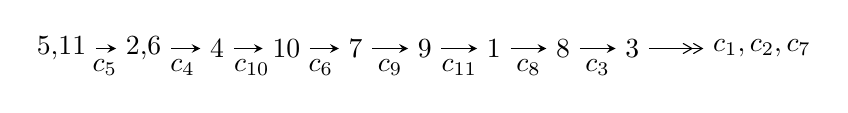
\begin{tikzpicture}[x=25pt, y=7pt]
	% node
	\node (A0) at (-1/8, 0) {5,11};
	\node (A1) at (17/16, 0) {2,6};
	\node (A2) at (17/8, 0) {4};
	\node (A3) at (25/8, 0) {10};
	\node (A4) at (33/8, 0) {7};
	\node (A5) at (41/8, 0) {9};
	\node (A6) at (49/8, 0) {1};
	\node (A7) at (57/8, 0) {8};
	\node (A8) at (65/8, 0) {3};
	\node (C1) at (1/2, -1) {$c_{5}$};
	\node (C2) at (13/8, -1) {$c_{4}$};
	\node (C3) at (21/8, -1) {$c_{10}$};
	\node (C4) at (29/8, -1) {$c_{6}$};
	\node (C5) at (37/8, -1) {$c_{9}$};
	\node (C6) at (45/8, -1) {$c_{11}$};
	\node (C7) at (53/8, -1) {$c_{8}$};
	\node (C8) at (61/8, -1) {$c_{3}$};
	\node (A9) at (10, 0) {$c_{1},c_{2},c_{7}$};

	% edge
	\draw[->,>=stealth]	
	(A0) edge (A1) (A1) edge (A2) (A2) edge (A3) (A3) edge (A4) (A4) edge (A5) (A5) edge (A6) (A6) edge (A7) (A7) edge (A8) ;
	\draw[->>,>={angle 60}]	
	(A8) edge (A9);
\end{tikzpicture} \\ 

\end{tabular} \\

\footnotetext{
The image of knot diagram is generated by the software ``\textbf{Draw programme}" developed by Andrew Bartholomew(\url{http://www.layer8.co.uk/maths/draw/index.htm\#Running-draw}), where we modified some parts for our purpose(\url{https://github.com/CATsTAILs/LinksPainter}).
}\phantom \\ \newline 
\centering \textbf{Ideals for irreducible components\footnotemark of $X_{\text{par}}$} 
 
\begin{align*}
I^u_{1}&=\langle 
u^{57}- u^{56}+\cdots+b+1,\;u^{59}-2 u^{58}+\cdots+a+3,\;u^{60}-2 u^{59}+\cdots+3 u-1\rangle \\
I^u_{2}&=\langle 
b+1,\;u^2+a- u+3,\;u^3- u^2+2 u-1\rangle \\
\\
\end{align*}
\raggedright * 2 irreducible components of $\dim_{\mathbb{C}}=0$, with total 63 representations.\\
\footnotetext{All coefficients of polynomials are rational numbers. But the coefficients are sometimes approximated in decimal forms when there is not enough margin.}
\newpage
\renewcommand{\arraystretch}{1}
\centering \section*{I. $I^u_{1}= \langle u^{57}- u^{56}+\cdots+b+1,\;u^{59}-2 u^{58}+\cdots+a+3,\;u^{60}-2 u^{59}+\cdots+3 u-1 \rangle$}
\flushleft \textbf{(i) Arc colorings}\\
\begin{tabular}{m{7pt} m{180pt} m{7pt} m{180pt} }
\flushright $a_{5}=$&$\begin{pmatrix}1\\0\end{pmatrix}$ \\
\flushright $a_{11}=$&$\begin{pmatrix}0\\u\end{pmatrix}$ \\
\flushright $a_{2}=$&$\begin{pmatrix}- u^{59}+2 u^{58}+\cdots+u-3\\- u^{57}+u^{56}+\cdots+u-1\end{pmatrix}$ \\
\flushright $a_{6}=$&$\begin{pmatrix}1\\u^2\end{pmatrix}$ \\
\flushright $a_{4}=$&$\begin{pmatrix}- u^{59}+2 u^{58}+\cdots+2 u-3\\- u^{57}+u^{56}+\cdots-3 u^3-1\end{pmatrix}$ \\
\flushright $a_{10}=$&$\begin{pmatrix}u\\u^3+u\end{pmatrix}$ \\
\flushright $a_{7}=$&$\begin{pmatrix}u^2+1\\u^4+2 u^2\end{pmatrix}$ \\
\flushright $a_{9}=$&$\begin{pmatrix}u^3+2 u\\u^3+u\end{pmatrix}$ \\
\flushright $a_{1}=$&$\begin{pmatrix}- u^7-4 u^5-4 u^3\\- u^7-3 u^5-2 u^3+u\end{pmatrix}$ \\
\flushright $a_{8}=$&$\begin{pmatrix}u^9+4 u^7+5 u^5+2 u^3+u\\u^{11}+5 u^9+8 u^7+3 u^5- u^3+u\end{pmatrix}$ \\
\flushright $a_{3}=$&$\begin{pmatrix}- u^{59}+2 u^{58}+\cdots- u^2-2\\- u^{57}+u^{56}+\cdots+u-1\end{pmatrix}$\\ \flushright $a_{3}=$&$\begin{pmatrix}- u^{59}+2 u^{58}+\cdots- u^2-2\\- u^{57}+u^{56}+\cdots+u-1\end{pmatrix}$\\&\end{tabular}
\flushleft \textbf{(ii) Obstruction class $= -1$}\\~\\
\flushleft \textbf{(iii) Cusp Shapes $= u^{59}-2 u^{58}+\cdots+8 u-3$}\\~\\
\newpage\renewcommand{\arraystretch}{1}
\flushleft \textbf{(iv) u-Polynomials at the component}\newline \\
\begin{tabular}{m{50pt}|m{274pt}}
Crossings & \hspace{64pt}u-Polynomials at each crossing \\
\hline $$\begin{aligned}c_{1},c_{4}\end{aligned}$$&$\begin{aligned}
&u^{60}-4 u^{59}+\cdots+4 u-1
\end{aligned}$\\
\hline $$\begin{aligned}c_{2}\end{aligned}$$&$\begin{aligned}
&u^{60}+32 u^{59}+\cdots+4 u+1
\end{aligned}$\\
\hline $$\begin{aligned}c_{3},c_{7}\end{aligned}$$&$\begin{aligned}
&u^{60}+u^{59}+\cdots+4 u+8
\end{aligned}$\\
\hline $$\begin{aligned}c_{5},c_{6},c_{10}\end{aligned}$$&$\begin{aligned}
&u^{60}-2 u^{59}+\cdots+3 u-1
\end{aligned}$\\
\hline $$\begin{aligned}c_{8}\end{aligned}$$&$\begin{aligned}
&u^{60}-21 u^{59}+\cdots-1040 u+64
\end{aligned}$\\
\hline $$\begin{aligned}c_{9}\end{aligned}$$&$\begin{aligned}
&u^{60}+2 u^{59}+\cdots+3 u-1
\end{aligned}$\\
\hline $$\begin{aligned}c_{11}\end{aligned}$$&$\begin{aligned}
&u^{60}-14 u^{59}+\cdots-1087 u+131
\end{aligned}$\\
\hline
\end{tabular}\\~\\
\newpage\renewcommand{\arraystretch}{1}
\flushleft \textbf{(v) Riley Polynomials at the component}\newline \\
\begin{tabular}{m{50pt}|m{274pt}}
Crossings & \hspace{64pt}Riley Polynomials at each crossing \\
\hline $$\begin{aligned}c_{1},c_{4}\end{aligned}$$&$\begin{aligned}
&y^{60}-32 y^{59}+\cdots-4 y+1
\end{aligned}$\\
\hline $$\begin{aligned}c_{2}\end{aligned}$$&$\begin{aligned}
&y^{60}-4 y^{59}+\cdots-32 y+1
\end{aligned}$\\
\hline $$\begin{aligned}c_{3},c_{7}\end{aligned}$$&$\begin{aligned}
&y^{60}-21 y^{59}+\cdots-1040 y+64
\end{aligned}$\\
\hline $$\begin{aligned}c_{5},c_{6},c_{10}\end{aligned}$$&$\begin{aligned}
&y^{60}+54 y^{59}+\cdots-7 y+1
\end{aligned}$\\
\hline $$\begin{aligned}c_{8}\end{aligned}$$&$\begin{aligned}
&y^{60}+31 y^{59}+\cdots-118016 y+4096
\end{aligned}$\\
\hline $$\begin{aligned}c_{9}\end{aligned}$$&$\begin{aligned}
&y^{60}-2 y^{59}+\cdots-7 y+1
\end{aligned}$\\
\hline $$\begin{aligned}c_{11}\end{aligned}$$&$\begin{aligned}
&y^{60}+10 y^{59}+\cdots+159609 y+17161
\end{aligned}$\\
\hline
\end{tabular}\\~\\
\newpage\flushleft \textbf{(vi) Complex Volumes and Cusp Shapes}
$$\begin{array}{c|c|c}  
\text{Solutions to }I^u_{1}& \I (\text{vol} + \sqrt{-1}CS) & \text{Cusp shape}\\
 \hline 
\begin{aligned}
u &= -0.272258 + 1.012540 I \\
a &= \phantom{-}1.93515 + 0.62774 I \\
b &= \phantom{-}1.147190 - 0.478763 I\end{aligned}
 & -2.04150 + 6.75419 I & -6.05975 - 7.03761 I \\ \hline\begin{aligned}
u &= -0.272258 - 1.012540 I \\
a &= \phantom{-}1.93515 - 0.62774 I \\
b &= \phantom{-}1.147190 + 0.478763 I\end{aligned}
 & -2.04150 - 6.75419 I & -6.05975 + 7.03761 I \\ \hline\begin{aligned}
u &= -0.156290 + 1.052030 I \\
a &= \phantom{-}0.095451 + 0.296346 I \\
b &= \phantom{-}0.098316 + 0.688037 I\end{aligned}
 & \phantom{-}0.89236 + 2.41054 I & -2.85789 - 3.50583 I \\ \hline\begin{aligned}
u &= -0.156290 - 1.052030 I \\
a &= \phantom{-}0.095451 - 0.296346 I \\
b &= \phantom{-}0.098316 - 0.688037 I\end{aligned}
 & \phantom{-}0.89236 - 2.41054 I & -2.85789 + 3.50583 I \\ \hline\begin{aligned}
u &= \phantom{-}0.102597 + 0.926022 I \\
a &= -1.92726 + 0.84189 I \\
b &= -1.169680 - 0.370214 I\end{aligned}
 & -2.71127 - 1.29749 I & -7.32877 + 0.87949 I \\ \hline\begin{aligned}
u &= \phantom{-}0.102597 - 0.926022 I \\
a &= -1.92726 - 0.84189 I \\
b &= -1.169680 + 0.370214 I\end{aligned}
 & -2.71127 + 1.29749 I & -7.32877 - 0.87949 I \\ \hline\begin{aligned}
u &= \phantom{-}0.362204 + 0.739680 I \\
a &= \phantom{-}1.398890 + 0.042352 I \\
b &= \phantom{-}1.157070 - 0.528981 I\end{aligned}
 & -1.51448 + 6.91671 I & -4.99151 - 4.33152 I \\ \hline\begin{aligned}
u &= \phantom{-}0.362204 - 0.739680 I \\
a &= \phantom{-}1.398890 - 0.042352 I \\
b &= \phantom{-}1.157070 + 0.528981 I\end{aligned}
 & -1.51448 - 6.91671 I & -4.99151 + 4.33152 I \\ \hline\begin{aligned}
u &= \phantom{-}0.739190 + 0.273449 I \\
a &= \phantom{-}2.83377 - 1.12471 I \\
b &= \phantom{-}1.183660 + 0.548618 I\end{aligned}
 & -3.14550 - 10.93560 I & -7.60991 + 8.98761 I \\ \hline\begin{aligned}
u &= \phantom{-}0.739190 - 0.273449 I \\
a &= \phantom{-}2.83377 + 1.12471 I \\
b &= \phantom{-}1.183660 - 0.548618 I\end{aligned}
 & -3.14550 + 10.93560 I & -7.60991 - 8.98761 I\\
 \hline 
 \end{array}$$\newpage$$\begin{array}{c|c|c}  
\text{Solutions to }I^u_{1}& \I (\text{vol} + \sqrt{-1}CS) & \text{Cusp shape}\\
 \hline 
\begin{aligned}
u &= \phantom{-}0.705650 + 0.274949 I \\
a &= -0.556763 - 0.943620 I \\
b &= \phantom{-}0.216325 - 0.833418 I\end{aligned}
 & -0.27172 - 5.84779 I & -4.34743 + 6.06110 I \\ \hline\begin{aligned}
u &= \phantom{-}0.705650 - 0.274949 I \\
a &= -0.556763 + 0.943620 I \\
b &= \phantom{-}0.216325 + 0.833418 I\end{aligned}
 & -0.27172 + 5.84779 I & -4.34743 - 6.06110 I \\ \hline\begin{aligned}
u &= -0.739469 + 0.157117 I \\
a &= \phantom{-}2.42529 + 0.98016 I \\
b &= \phantom{-}1.123680 + 0.435823 I\end{aligned}
 & -4.64706 - 2.94332 I & -9.69548 + 3.11009 I \\ \hline\begin{aligned}
u &= -0.739469 - 0.157117 I \\
a &= \phantom{-}2.42529 - 0.98016 I \\
b &= \phantom{-}1.123680 - 0.435823 I\end{aligned}
 & -4.64706 + 2.94332 I & -9.69548 - 3.11009 I \\ \hline\begin{aligned}
u &= -0.701322 + 0.243359 I \\
a &= -2.80040 - 1.59166 I \\
b &= -1.129360 + 0.462569 I\end{aligned}
 & -4.44900 + 4.80272 I & -9.53100 - 5.34375 I \\ \hline\begin{aligned}
u &= -0.701322 - 0.243359 I \\
a &= -2.80040 + 1.59166 I \\
b &= -1.129360 - 0.462569 I\end{aligned}
 & -4.44900 - 4.80272 I & -9.53100 + 5.34375 I \\ \hline\begin{aligned}
u &= \phantom{-}0.691544 + 0.218830 I \\
a &= -2.61676 + 0.96703 I \\
b &= -1.228960 + 0.314277 I\end{aligned}
 & -4.78959 - 2.10958 I & -9.89618 + 4.41005 I \\ \hline\begin{aligned}
u &= \phantom{-}0.691544 - 0.218830 I \\
a &= -2.61676 - 0.96703 I \\
b &= -1.228960 - 0.314277 I\end{aligned}
 & -4.78959 + 2.10958 I & -9.89618 - 4.41005 I \\ \hline\begin{aligned}
u &= -0.150600 + 0.704962 I \\
a &= -1.51108 + 0.72061 I \\
b &= -1.130100 - 0.383816 I\end{aligned}
 & -2.66735 - 1.26395 I & -6.69853 + 0.15559 I \\ \hline\begin{aligned}
u &= -0.150600 - 0.704962 I \\
a &= -1.51108 - 0.72061 I \\
b &= -1.130100 + 0.383816 I\end{aligned}
 & -2.66735 + 1.26395 I & -6.69853 - 0.15559 I\\
 \hline 
 \end{array}$$\newpage$$\begin{array}{c|c|c}  
\text{Solutions to }I^u_{1}& \I (\text{vol} + \sqrt{-1}CS) & \text{Cusp shape}\\
 \hline 
\begin{aligned}
u &= -0.245563 + 1.262290 I \\
a &= \phantom{-}1.207160 + 0.477268 I \\
b &= \phantom{-}0.712663 - 0.173753 I\end{aligned}
 & \phantom{-}2.15190 + 3.30985 I & \phantom{-0.000000 } 0 \\ \hline\begin{aligned}
u &= -0.245563 - 1.262290 I \\
a &= \phantom{-}1.207160 - 0.477268 I \\
b &= \phantom{-}0.712663 + 0.173753 I\end{aligned}
 & \phantom{-}2.15190 - 3.30985 I & \phantom{-0.000000 } 0 \\ \hline\begin{aligned}
u &= \phantom{-}0.313312 + 0.634127 I \\
a &= \phantom{-}0.406095 + 0.033528 I \\
b &= \phantom{-}0.231815 + 0.743223 I\end{aligned}
 & \phantom{-}1.19086 + 2.11650 I & -1.10142 - 0.94504 I \\ \hline\begin{aligned}
u &= \phantom{-}0.313312 - 0.634127 I \\
a &= \phantom{-}0.406095 - 0.033528 I \\
b &= \phantom{-}0.231815 - 0.743223 I\end{aligned}
 & \phantom{-}1.19086 - 2.11650 I & -1.10142 + 0.94504 I \\ \hline\begin{aligned}
u &= \phantom{-}0.593362 + 0.375996 I \\
a &= \phantom{-}1.44574 - 0.93956 I \\
b &= \phantom{-}0.826187 + 0.623051 I\end{aligned}
 & \phantom{-}3.02257 - 4.24450 I & -1.33904 + 7.25011 I \\ \hline\begin{aligned}
u &= \phantom{-}0.593362 - 0.375996 I \\
a &= \phantom{-}1.44574 + 0.93956 I \\
b &= \phantom{-}0.826187 - 0.623051 I\end{aligned}
 & \phantom{-}3.02257 + 4.24450 I & -1.33904 - 7.25011 I \\ \hline\begin{aligned}
u &= -0.651026 + 0.178717 I \\
a &= \phantom{-}0.833384 - 0.653334 I \\
b &= -0.075209 - 0.564522 I\end{aligned}
 & -1.64038 + 0.76431 I & -6.82050 - 1.17334 I \\ \hline\begin{aligned}
u &= -0.651026 - 0.178717 I \\
a &= \phantom{-}0.833384 + 0.653334 I \\
b &= -0.075209 + 0.564522 I\end{aligned}
 & -1.64038 - 0.76431 I & -6.82050 + 1.17334 I \\ \hline\begin{aligned}
u &= \phantom{-}0.514134 + 0.433646 I \\
a &= \phantom{-}0.120502 - 0.319390 I \\
b &= \phantom{-}0.725195 - 0.626130 I\end{aligned}
 & \phantom{-}3.31167 + 0.60747 I & \phantom{-}0.058994 + 0.358835 I \\ \hline\begin{aligned}
u &= \phantom{-}0.514134 - 0.433646 I \\
a &= \phantom{-}0.120502 + 0.319390 I \\
b &= \phantom{-}0.725195 + 0.626130 I\end{aligned}
 & \phantom{-}3.31167 - 0.60747 I & \phantom{-}0.058994 - 0.358835 I\\
 \hline 
 \end{array}$$\newpage$$\begin{array}{c|c|c}  
\text{Solutions to }I^u_{1}& \I (\text{vol} + \sqrt{-1}CS) & \text{Cusp shape}\\
 \hline 
\begin{aligned}
u &= -0.667151\phantom{ +0.000000I} \\
a &= \phantom{-}1.87106\phantom{ +0.000000I} \\
b &= \phantom{-}0.617384\phantom{ +0.000000I}\end{aligned}
 & -1.74355\phantom{ +0.000000I} & -3.65290\phantom{ +0.000000I} \\ \hline\begin{aligned}
u &= \phantom{-}0.146423 + 1.356920 I \\
a &= -1.11641 + 0.87341 I \\
b &= -1.211750 - 0.122488 I\end{aligned}
 & \phantom{-}2.27680 - 1.86506 I & \phantom{-0.000000 } 0 \\ \hline\begin{aligned}
u &= \phantom{-}0.146423 - 1.356920 I \\
a &= -1.11641 - 0.87341 I \\
b &= -1.211750 + 0.122488 I\end{aligned}
 & \phantom{-}2.27680 + 1.86506 I & \phantom{-0.000000 } 0 \\ \hline\begin{aligned}
u &= -0.298418 + 1.347350 I \\
a &= \phantom{-}0.950662 + 0.883761 I \\
b &= \phantom{-}1.102840 + 0.401160 I\end{aligned}
 & \phantom{-}0.089664 + 0.805813 I & \phantom{-0.000000 } 0 \\ \hline\begin{aligned}
u &= -0.298418 - 1.347350 I \\
a &= \phantom{-}0.950662 - 0.883761 I \\
b &= \phantom{-}1.102840 - 0.401160 I\end{aligned}
 & \phantom{-}0.089664 - 0.805813 I & \phantom{-0.000000 } 0 \\ \hline\begin{aligned}
u &= -0.112811 + 1.380760 I \\
a &= \phantom{-}0.088761 + 1.367980 I \\
b &= -0.973157 - 0.442087 I\end{aligned}
 & \phantom{-}3.11222 - 0.32948 I & \phantom{-0.000000 } 0 \\ \hline\begin{aligned}
u &= -0.112811 - 1.380760 I \\
a &= \phantom{-}0.088761 - 1.367980 I \\
b &= -0.973157 + 0.442087 I\end{aligned}
 & \phantom{-}3.11222 + 0.32948 I & \phantom{-0.000000 } 0 \\ \hline\begin{aligned}
u &= -0.181790 + 1.380090 I \\
a &= \phantom{-}0.51009 - 1.34681 I \\
b &= -0.578631 + 0.449363 I\end{aligned}
 & \phantom{-}4.27304 + 3.48079 I & \phantom{-0.000000 } 0 \\ \hline\begin{aligned}
u &= -0.181790 - 1.380090 I \\
a &= \phantom{-}0.51009 + 1.34681 I \\
b &= -0.578631 - 0.449363 I\end{aligned}
 & \phantom{-}4.27304 - 3.48079 I & \phantom{-0.000000 } 0 \\ \hline\begin{aligned}
u &= -0.252426 + 1.375440 I \\
a &= \phantom{-}1.054820 + 0.112572 I \\
b &= -0.213723 - 0.598525 I\end{aligned}
 & \phantom{-}3.31453 + 4.03685 I & \phantom{-0.000000 } 0\\
 \hline 
 \end{array}$$\newpage$$\begin{array}{c|c|c}  
\text{Solutions to }I^u_{1}& \I (\text{vol} + \sqrt{-1}CS) & \text{Cusp shape}\\
 \hline 
\begin{aligned}
u &= -0.252426 - 1.375440 I \\
a &= \phantom{-}1.054820 - 0.112572 I \\
b &= -0.213723 + 0.598525 I\end{aligned}
 & \phantom{-}3.31453 - 4.03685 I & \phantom{-0.000000 } 0 \\ \hline\begin{aligned}
u &= \phantom{-}0.272964 + 1.386080 I \\
a &= -1.045560 + 0.896556 I \\
b &= -1.260740 + 0.293725 I\end{aligned}
 & \phantom{-}0.31494 - 5.61200 I & \phantom{-0.000000 } 0 \\ \hline\begin{aligned}
u &= \phantom{-}0.272964 - 1.386080 I \\
a &= -1.045560 - 0.896556 I \\
b &= -1.260740 - 0.293725 I\end{aligned}
 & \phantom{-}0.31494 + 5.61200 I & \phantom{-0.000000 } 0 \\ \hline\begin{aligned}
u &= -0.27784 + 1.39711 I \\
a &= -1.46445 - 2.26687 I \\
b &= -1.121330 + 0.494109 I\end{aligned}
 & \phantom{-}0.77544 + 8.36220 I & \phantom{-0.000000 } 0 \\ \hline\begin{aligned}
u &= -0.27784 - 1.39711 I \\
a &= -1.46445 + 2.26687 I \\
b &= -1.121330 - 0.494109 I\end{aligned}
 & \phantom{-}0.77544 - 8.36220 I & \phantom{-0.000000 } 0 \\ \hline\begin{aligned}
u &= \phantom{-}0.11177 + 1.42352 I \\
a &= \phantom{-}0.003244 - 0.724114 I \\
b &= \phantom{-}0.361594 + 0.782628 I\end{aligned}
 & \phantom{-}7.44712 + 0.69473 I & \phantom{-0.000000 } 0 \\ \hline\begin{aligned}
u &= \phantom{-}0.11177 - 1.42352 I \\
a &= \phantom{-}0.003244 + 0.724114 I \\
b &= \phantom{-}0.361594 - 0.782628 I\end{aligned}
 & \phantom{-}7.44712 - 0.69473 I & \phantom{-0.000000 } 0 \\ \hline\begin{aligned}
u &= \phantom{-}0.27859 + 1.41128 I \\
a &= -0.929433 - 0.027526 I \\
b &= \phantom{-}0.233048 - 0.870544 I\end{aligned}
 & \phantom{-}5.10898 - 9.43023 I & \phantom{-0.000000 } 0 \\ \hline\begin{aligned}
u &= \phantom{-}0.27859 - 1.41128 I \\
a &= -0.929433 + 0.027526 I \\
b &= \phantom{-}0.233048 + 0.870544 I\end{aligned}
 & \phantom{-}5.10898 + 9.43023 I & \phantom{-0.000000 } 0 \\ \hline\begin{aligned}
u &= \phantom{-}0.07750 + 1.43810 I \\
a &= \phantom{-}0.274235 + 0.847102 I \\
b &= \phantom{-}1.113070 - 0.571356 I\end{aligned}
 & \phantom{-}5.22134 + 5.76496 I & \phantom{-0.000000 } 0\\
 \hline 
 \end{array}$$\newpage$$\begin{array}{c|c|c}  
\text{Solutions to }I^u_{1}& \I (\text{vol} + \sqrt{-1}CS) & \text{Cusp shape}\\
 \hline 
\begin{aligned}
u &= \phantom{-}0.07750 - 1.43810 I \\
a &= \phantom{-}0.274235 - 0.847102 I \\
b &= \phantom{-}1.113070 + 0.571356 I\end{aligned}
 & \phantom{-}5.22134 - 5.76496 I & \phantom{-0.000000 } 0 \\ \hline\begin{aligned}
u &= \phantom{-}0.29362 + 1.41349 I \\
a &= \phantom{-}1.61836 - 1.90667 I \\
b &= \phantom{-}1.192200 + 0.565015 I\end{aligned}
 & \phantom{-}2.2343 - 14.6854 I & \phantom{-0.000000 } 0 \\ \hline\begin{aligned}
u &= \phantom{-}0.29362 - 1.41349 I \\
a &= \phantom{-}1.61836 + 1.90667 I \\
b &= \phantom{-}1.192200 - 0.565015 I\end{aligned}
 & \phantom{-}2.2343 + 14.6854 I & \phantom{-0.000000 } 0 \\ \hline\begin{aligned}
u &= \phantom{-}0.19005 + 1.43268 I \\
a &= -0.563532 + 0.432636 I \\
b &= \phantom{-}0.708476 - 0.712296 I\end{aligned}
 & \phantom{-}9.23623 - 1.96231 I & \phantom{-0.000000 } 0 \\ \hline\begin{aligned}
u &= \phantom{-}0.19005 - 1.43268 I \\
a &= -0.563532 - 0.432636 I \\
b &= \phantom{-}0.708476 + 0.712296 I\end{aligned}
 & \phantom{-}9.23623 + 1.96231 I & \phantom{-0.000000 } 0 \\ \hline\begin{aligned}
u &= \phantom{-}0.22072 + 1.43184 I \\
a &= \phantom{-}0.55993 - 1.54260 I \\
b &= \phantom{-}0.857884 + 0.678909 I\end{aligned}
 & \phantom{-}8.80345 - 7.21631 I & \phantom{-0.000000 } 0 \\ \hline\begin{aligned}
u &= \phantom{-}0.22072 - 1.43184 I \\
a &= \phantom{-}0.55993 + 1.54260 I \\
b &= \phantom{-}0.857884 - 0.678909 I\end{aligned}
 & \phantom{-}8.80345 + 7.21631 I & \phantom{-0.000000 } 0 \\ \hline\begin{aligned}
u &= -0.434286 + 0.236524 I \\
a &= \phantom{-}0.227567 - 1.379360 I \\
b &= -0.654919 + 0.246891 I\end{aligned}
 & -0.85637 + 1.13107 I & -6.00125 - 6.01444 I \\ \hline\begin{aligned}
u &= -0.434286 - 0.236524 I \\
a &= \phantom{-}0.227567 + 1.379360 I \\
b &= -0.654919 - 0.246891 I\end{aligned}
 & -0.85637 - 1.13107 I & -6.00125 + 6.01444 I \\ \hline\begin{aligned}
u &= \phantom{-}0.388108\phantom{ +0.000000I} \\
a &= -3.78596\phantom{ +0.000000I} \\
b &= -1.10470\phantom{ +0.000000I}\end{aligned}
 & -2.19031\phantom{ +0.000000I} & \phantom{-}0.722320\phantom{ +0.000000I}\\
 \hline 
 \end{array}$$\newpage\newpage\renewcommand{\arraystretch}{1}
\centering \section*{II. $I^u_{2}= \langle b+1,\;u^2+a- u+3,\;u^3- u^2+2 u-1 \rangle$}
\flushleft \textbf{(i) Arc colorings}\\
\begin{tabular}{m{7pt} m{180pt} m{7pt} m{180pt} }
\flushright $a_{5}=$&$\begin{pmatrix}1\\0\end{pmatrix}$ \\
\flushright $a_{11}=$&$\begin{pmatrix}0\\u\end{pmatrix}$ \\
\flushright $a_{2}=$&$\begin{pmatrix}- u^2+u-3\\-1\end{pmatrix}$ \\
\flushright $a_{6}=$&$\begin{pmatrix}1\\u^2\end{pmatrix}$ \\
\flushright $a_{4}=$&$\begin{pmatrix}- u^2+u-2\\-1\end{pmatrix}$ \\
\flushright $a_{10}=$&$\begin{pmatrix}u\\u^2- u+1\end{pmatrix}$ \\
\flushright $a_{7}=$&$\begin{pmatrix}u^2+1\\u^2- u+1\end{pmatrix}$ \\
\flushright $a_{9}=$&$\begin{pmatrix}u^2+1\\u^2- u+1\end{pmatrix}$ \\
\flushright $a_{1}=$&$\begin{pmatrix}-1\\0\end{pmatrix}$ \\
\flushright $a_{8}=$&$\begin{pmatrix}u^2+1\\u^2- u+1\end{pmatrix}$ \\
\flushright $a_{3}=$&$\begin{pmatrix}- u^2+u-2\\-1\end{pmatrix}$\\ \flushright $a_{3}=$&$\begin{pmatrix}- u^2+u-2\\-1\end{pmatrix}$\\&\end{tabular}
\flushleft \textbf{(ii) Obstruction class $= 1$}\\~\\
\flushleft \textbf{(iii) Cusp Shapes $= -5 u^2+4 u-16$}\\~\\
\newpage\renewcommand{\arraystretch}{1}
\flushleft \textbf{(iv) u-Polynomials at the component}\newline \\
\begin{tabular}{m{50pt}|m{274pt}}
Crossings & \hspace{64pt}u-Polynomials at each crossing \\
\hline $$\begin{aligned}c_{1}\end{aligned}$$&$\begin{aligned}
&(u-1)^3
\end{aligned}$\\
\hline $$\begin{aligned}c_{2},c_{4}\end{aligned}$$&$\begin{aligned}
&(u+1)^3
\end{aligned}$\\
\hline $$\begin{aligned}c_{3},c_{7},c_{8}\end{aligned}$$&$\begin{aligned}
&u^3
\end{aligned}$\\
\hline $$\begin{aligned}c_{5},c_{6}\end{aligned}$$&$\begin{aligned}
&u^3- u^2+2 u-1
\end{aligned}$\\
\hline $$\begin{aligned}c_{9},c_{11}\end{aligned}$$&$\begin{aligned}
&u^3- u^2+1
\end{aligned}$\\
\hline $$\begin{aligned}c_{10}\end{aligned}$$&$\begin{aligned}
&u^3+u^2+2 u+1
\end{aligned}$\\
\hline
\end{tabular}\\~\\
\newpage\renewcommand{\arraystretch}{1}
\flushleft \textbf{(v) Riley Polynomials at the component}\newline \\
\begin{tabular}{m{50pt}|m{274pt}}
Crossings & \hspace{64pt}Riley Polynomials at each crossing \\
\hline $$\begin{aligned}c_{1},c_{2},c_{4}\end{aligned}$$&$\begin{aligned}
&(y-1)^3
\end{aligned}$\\
\hline $$\begin{aligned}c_{3},c_{7},c_{8}\end{aligned}$$&$\begin{aligned}
&y^3
\end{aligned}$\\
\hline $$\begin{aligned}c_{5},c_{6},c_{10}\end{aligned}$$&$\begin{aligned}
&y^3+3 y^2+2 y-1
\end{aligned}$\\
\hline $$\begin{aligned}c_{9},c_{11}\end{aligned}$$&$\begin{aligned}
&y^3- y^2+2 y-1
\end{aligned}$\\
\hline
\end{tabular}\\~\\
\newpage\flushleft \textbf{(vi) Complex Volumes and Cusp Shapes}
$$\begin{array}{c|c|c}  
\text{Solutions to }I^u_{2}& \I (\text{vol} + \sqrt{-1}CS) & \text{Cusp shape}\\
 \hline 
\begin{aligned}
u &= \phantom{-}0.215080 + 1.307140 I \\
a &= -1.122560 + 0.744862 I \\
b &= -1.00000\phantom{ +0.000000I}\end{aligned}
 & \phantom{-}1.37919 - 2.82812 I & -6.82789 + 2.41717 I \\ \hline\begin{aligned}
u &= \phantom{-}0.215080 - 1.307140 I \\
a &= -1.122560 - 0.744862 I \\
b &= -1.00000\phantom{ +0.000000I}\end{aligned}
 & \phantom{-}1.37919 + 2.82812 I & -6.82789 - 2.41717 I \\ \hline\begin{aligned}
u &= \phantom{-}0.569840\phantom{ +0.000000I} \\
a &= -2.75488\phantom{ +0.000000I} \\
b &= -1.00000\phantom{ +0.000000I}\end{aligned}
 & -2.75839\phantom{ +0.000000I} & -15.3440\phantom{ +0.000000I}\\
 \hline 
 \end{array}$$\newpage
\newpage\renewcommand{\arraystretch}{1}
\centering \section*{ III. u-Polynomials}
\begin{tabular}{m{50pt}|m{274pt}}
Crossings & \hspace{64pt}u-Polynomials at each crossing \\
\hline $$\begin{aligned}c_{1}\end{aligned}$$&$\begin{aligned}
&((u-1)^3)(u^{60}-4 u^{59}+\cdots+4 u-1)
\end{aligned}$\\
\hline $$\begin{aligned}c_{2}\end{aligned}$$&$\begin{aligned}
&((u+1)^3)(u^{60}+32 u^{59}+\cdots+4 u+1)
\end{aligned}$\\
\hline $$\begin{aligned}c_{3},c_{7}\end{aligned}$$&$\begin{aligned}
&u^3(u^{60}+u^{59}+\cdots+4 u+8)
\end{aligned}$\\
\hline $$\begin{aligned}c_{4}\end{aligned}$$&$\begin{aligned}
&((u+1)^3)(u^{60}-4 u^{59}+\cdots+4 u-1)
\end{aligned}$\\
\hline $$\begin{aligned}c_{5},c_{6}\end{aligned}$$&$\begin{aligned}
&(u^3- u^2+2 u-1)(u^{60}-2 u^{59}+\cdots+3 u-1)
\end{aligned}$\\
\hline $$\begin{aligned}c_{8}\end{aligned}$$&$\begin{aligned}
&u^3(u^{60}-21 u^{59}+\cdots-1040 u+64)
\end{aligned}$\\
\hline $$\begin{aligned}c_{9}\end{aligned}$$&$\begin{aligned}
&(u^3- u^2+1)(u^{60}+2 u^{59}+\cdots+3 u-1)
\end{aligned}$\\
\hline $$\begin{aligned}c_{10}\end{aligned}$$&$\begin{aligned}
&(u^3+u^2+2 u+1)(u^{60}-2 u^{59}+\cdots+3 u-1)
\end{aligned}$\\
\hline $$\begin{aligned}c_{11}\end{aligned}$$&$\begin{aligned}
&(u^3- u^2+1)(u^{60}-14 u^{59}+\cdots-1087 u+131)
\end{aligned}$\\
\hline
\end{tabular}\newpage\renewcommand{\arraystretch}{1}
\centering \section*{ IV. Riley Polynomials}
\begin{tabular}{m{50pt}|m{274pt}}
Crossings & \hspace{64pt}Riley Polynomials at each crossing \\
\hline $$\begin{aligned}c_{1},c_{4}\end{aligned}$$&$\begin{aligned}
&((y-1)^3)(y^{60}-32 y^{59}+\cdots-4 y+1)
\end{aligned}$\\
\hline $$\begin{aligned}c_{2}\end{aligned}$$&$\begin{aligned}
&((y-1)^3)(y^{60}-4 y^{59}+\cdots-32 y+1)
\end{aligned}$\\
\hline $$\begin{aligned}c_{3},c_{7}\end{aligned}$$&$\begin{aligned}
&y^3(y^{60}-21 y^{59}+\cdots-1040 y+64)
\end{aligned}$\\
\hline $$\begin{aligned}c_{5},c_{6},c_{10}\end{aligned}$$&$\begin{aligned}
&(y^3+3 y^2+2 y-1)(y^{60}+54 y^{59}+\cdots-7 y+1)
\end{aligned}$\\
\hline $$\begin{aligned}c_{8}\end{aligned}$$&$\begin{aligned}
&y^3(y^{60}+31 y^{59}+\cdots-118016 y+4096)
\end{aligned}$\\
\hline $$\begin{aligned}c_{9}\end{aligned}$$&$\begin{aligned}
&(y^3- y^2+2 y-1)(y^{60}-2 y^{59}+\cdots-7 y+1)
\end{aligned}$\\
\hline $$\begin{aligned}c_{11}\end{aligned}$$&$\begin{aligned}
&(y^3- y^2+2 y-1)(y^{60}+10 y^{59}+\cdots+159609 y+17161)
\end{aligned}$\\
\hline
\end{tabular}
\vskip 2pc
\end{document}